\chapter{Provocări și aspecte practice ale procesului de lucru}
\begin{sloppypar}

În acest capitol aș dori să detaliez unele aspecte care consider că sunt destul de importante de menționat și unele provocări întâlnite pe parcursul procesului de dezvoltare. \par
Pentru realizarea proiectului am folosit Visual Studio ca mediu de dezolvare, acesta oferind o interfață intuitivă, dar și multe alte funcționalități care au facilitat procesul de dezvoltare și care sunt disponibile prin intermediul serverului Dafny. Acesta furnizează instrumente pentru evidențierea sintaxei, verificarea codului pe măsură ce instrucțiunile sunt tastate și feedback vizual pentru starea curentă a verificării formale a programului. \cite{leino2021dafny} \par
Aceasta din urmă a fost, in mod special, foarte folositor pentru a mă asigura că verificarea formală a metodelor și a lemelor a trecut cu succes. Evidențierea verificării poate fi observată în partea din stânga a editorului (săgeata 1):
\begin{figure}[!ht]
    \centering
    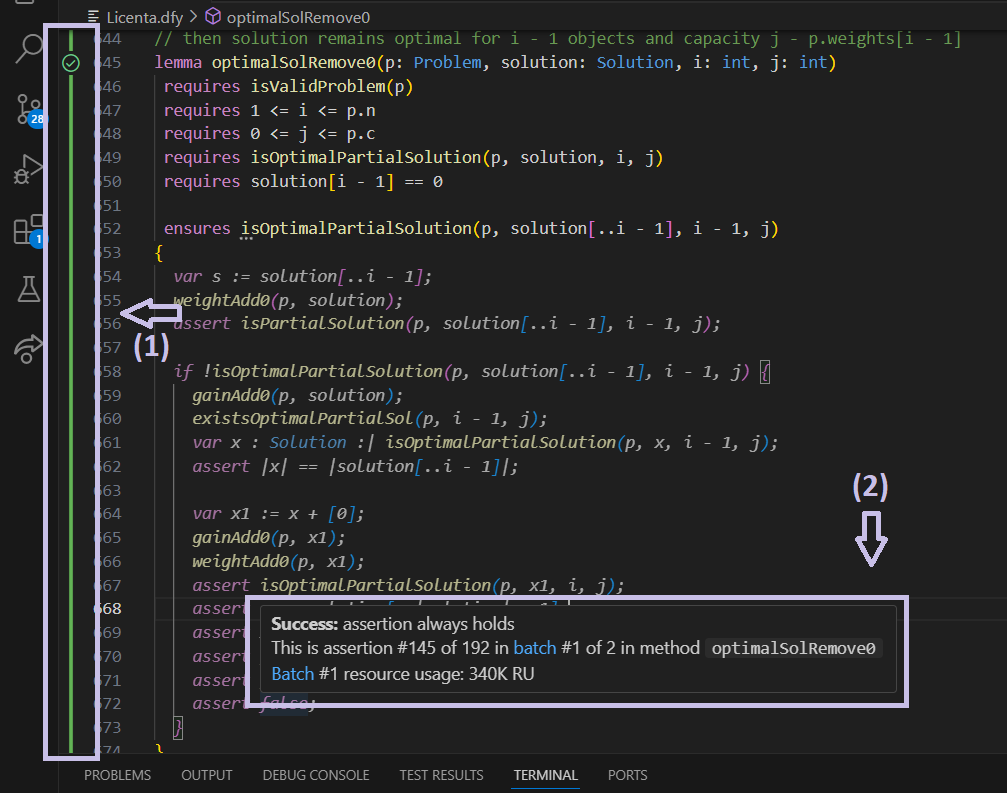
\includegraphics[width=0.6\linewidth]{images/imageVerificationSucceeded.png}
\end{figure}
 \par De exemplu, pentru lema \formatText{optimalSolRemove0} Dafny a reușit să verifice cu succes corectitudinea acesteia, iar acest lucru este evidențiat printr-o bară verticală de culoare verde pe toată lungimea declarației acesteia. În funcție de starea procesului de verificare, această bară își va schimba stilul în mod dinamic pentru a ajuta programatorul în procesul de dezvoltare al codului.
 \par De asemenea, dacă plasăm cursorul peste o instrucțiune, o fereastră pop-up apare în care putem afla informații despre stadiul verificării acesteia (săgeata 2). Acest lucru este de ajutor mai mult în cazul invarianților pentru a afla dacă verificatorul nu poate demonstra corectitudinea acestuia înainte de execuția buclei sau în timpul acesteia. \par
 Pentru a rula algoritmul, avem două variante:
 \begin{itemize}
     \item click dreapta în fișierul ce se dorește a fi rulat și alegem \texttt{Dafny} $\rightarrow$ \texttt{Dafny:Run} (sau \texttt{F5})
     \item din linia de comandă se poate executa următoarea comanda: \texttt{dafny run Licenta.dfy} (mai multe opțiuni de control al verificării pot fi adăugate, precum \texttt{--allow-warnings})
 \end{itemize}
 \par
Una dintre cele mai comune provocări pe care le-am întâmpinat pe parcursul procesului de implementare a fost depășirea timpului de răspuns alocat pentru verificarea unei leme sau a unei metode, care poate apărea atunci când unele specificații nu sunt complete sau când logica demonstrației este mult prea complexă pentru verificator, dar există și cazuri în care acesta se pierde încercând să demonstreze lanțuri inutile de raționament. \cite{verification_optimization} În astfel de cazuri am avut la îndemană următoarele posibilități:
\begin{itemize}
    \item Utilizarea instrucțiunilor \texttt{assert}: acestea sunt folosite pentru a verifica valoarea de adevăr a unei expresii logice necesare în demonstrație. Cu ajutorul acestora am verificat dacă Dafny poate aproba raționamentul pe care l-am aplicat în demonstrarea postcondițiilor deoarece de foarte multe ori a fost nevoie să ghidez verificatorul spre o anumită direcție logică, dar și unele proprietăți care trebuiau să fie adevărate după apelarea unor leme pentru a continua verificarea. Un exemplu foarte bun pentru ambele cazuri este lema \formatText{gainAddTooBig}:
   \begin{Verbatim}[commandchars=\\\{\}]
\PY{k+kd}{lemma} \PY{n+nf}{gainAddTooBig}\PY{p}{(}\PY{n}{p}\PY{p}{:} \PY{n}{Problem}\PY{p}{,} \PY{n}{solution}\PY{p}{:} \PY{n}{Solution}\PY{p}{,} 
    \PY{n}{i}\PY{p}{:} \PY{k+kt}{int}\PY{p}{,} \PY{n}{j}\PY{p}{:} \PY{k+kt}{int}\PY{p}{)} 
 \PY{p}{..}\PY{p}{.}
 \PY{k}{requires} \PY{n}{isPartialSolution}\PY{p}{(}\PY{n}{p}\PY{p}{,} \PY{n}{solution}\PY{p}{,} \PY{n}{i}\PY{p}{,} \PY{n}{j}\PY{p}{)}
 \PY{k}{requires} \PY{n}{p}\PY{p}{.}\PY{n}{weights}\PY{p}{[}\PY{n}{i} \PY{o}{\PYZhy{}} \PY{l+m+mi}{1}\PY{p}{]} \PY{o}{\PYZgt{}} \PY{n}{j}
 \PY{k}{ensures} \PY{n}{solution}\PY{p}{[}\PY{n}{i} \PY{o}{\PYZhy{}} \PY{l+m+mi}{1}\PY{p}{]} \PY{o}{==} \PY{l+m+mi}{0}
 \PY{k}{ensures} \PY{n}{gain}\PY{p}{(}\PY{n}{p}\PY{p}{,} \PY{n}{solution}\PY{p}{[}\PY{p}{..}\PY{n}{i} \PY{o}{\PYZhy{}} \PY{l+m+mi}{1}\PY{p}{]}\PY{p}{)} \PY{o}{==} \PY{n}{gain}\PY{p}{(}\PY{n}{p}\PY{p}{,} \PY{n}{solution}\PY{p}{)}
 \PY{p}{\PYZob{}}
    \PY{k}{if} \PY{n}{solution}\PY{p}{[}\PY{n}{i} \PY{o}{\PYZhy{}} \PY{l+m+mi}{1}\PY{p}{]} \PY{o}{==} \PY{l+m+mi}{1} \PY{p}{\PYZob{}}
      \PY{k}{assert} \PY{n}{computeWeight}\PY{p}{(}\PY{n}{p}\PY{p}{,} \PY{n}{solution}\PY{p}{,} \PY{o}{|}\PY{n}{solution}\PY{o}{|} \PY{o}{\PYZhy{}} \PY{l+m+mi}{1}\PY{p}{)} \PY{o}{==} 
        \PY{n}{computeWeight}\PY{p}{(}\PY{n}{p}\PY{p}{,} \PY{n}{solution}\PY{p}{,} \PY{o}{|}\PY{n}{solution}\PY{p}{[}\PY{p}{..}\PY{n}{i}\PY{p}{]}\PY{o}{|} \PY{o}{\PYZhy{}} \PY{l+m+mi}{1}\PY{p}{)} \PY{o}{+} 
        \PY{n}{p}\PY{p}{.}\PY{n}{weights}\PY{p}{[}\PY{n}{i} \PY{o}{\PYZhy{}} \PY{l+m+mi}{1}\PY{p}{]}\PY{p}{;}
      \PY{k}{assert} \PY{n}{weight}\PY{p}{(}\PY{n}{p}\PY{p}{,} \PY{n}{solution}\PY{p}{)} \PY{o}{\PYZgt{}=} \PY{n}{p}\PY{p}{.}\PY{n}{weights}\PY{p}{[}\PY{n}{i} \PY{o}{\PYZhy{}} \PY{l+m+mi}{1}\PY{p}{]} \PY{o}{\PYZgt{}} \PY{n}{j}\PY{p}{;}
      \PY{k}{assert} \PY{err}{!}\PY{n}{isPartialSolution}\PY{p}{(}\PY{n}{p}\PY{p}{,} \PY{n}{solution}\PY{p}{,} \PY{n}{i}\PY{p}{,} \PY{n}{j}\PY{p}{)}\PY{p}{;}
      \PY{k}{assert} \PY{k+kc}{false}\PY{p}{;}
    \PY{p}{\PYZcb{}}
    \PY{k}{assert} \PY{n}{solution}\PY{p}{[}\PY{n}{i} \PY{o}{\PYZhy{}} \PY{l+m+mi}{1}\PY{p}{]} \PY{o}{==} \PY{l+m+mi}{0}\PY{p}{;}
    \PY{n}{computeGainAdd0}\PY{p}{(}\PY{n}{p}\PY{p}{,} \PY{n}{solution}\PY{p}{,} \PY{o}{|}\PY{n}{solution}\PY{o}{|} \PY{o}{\PYZhy{}} \PY{l+m+mi}{2}\PY{p}{)}\PY{p}{;}
    \PY{k}{assert} \PY{n}{gain}\PY{p}{(}\PY{n}{p}\PY{p}{,} \PY{n}{solution}\PY{p}{[}\PY{p}{..}\PY{n}{i} \PY{o}{\PYZhy{}} \PY{l+m+mi}{1}\PY{p}{]}\PY{p}{)} \PY{o}{==} \PY{n}{gain}\PY{p}{(}\PY{n}{p}\PY{p}{,} \PY{n}{solution}\PY{p}{)}\PY{p}{;}
\PY{p}{\PYZcb{}}
\end{Verbatim}
    unde \texttt{assert-urile} din instrucțiunea \textit{if} urmăresc să ajungem la o contradicție prin faptul că soluția nu are cum să fie parțială dacă greutatea obiectului depășește capacitatea $j$, propoziție care este falsă deoarece avem o precondiție care asigură exact acest lucru, iar instrucțiunea 
    \begin{Verbatim}[commandchars=\\\{\}]
\PY{k}{assert} \PY{n}{gain}\PY{p}{(}\PY{n}{p}\PY{p}{,} \PY{n}{solution}\PY{p}{[}\PY{p}{..}\PY{n}{i} \PY{o}{\PYZhy{}} \PY{l+m+mi}{1}\PY{p}{]}\PY{p}{)} \PY{o}{==} \PY{n}{gain}\PY{p}{(}\PY{n}{p}\PY{p}{,} \PY{n}{solution}\PY{p}{)}\PY{p}{;}
\end{Verbatim}
    se asigură că după apelarea lemei computeGainAdd0 verificatorul știe că profitul unei soluții rămâne neschimbat dacă eliminăm ultimul element de 0 din soluție. \par
    \hspace{2mm} De asemenea, folosind structura \texttt{assert ... by} putem reduce sarcina verificatorului deoarece pașii din acest bloc de instrucțiuni sunt "uitați" după verificarea condiției din assert:
    \begin{Verbatim}[commandchars=\\\{\}]
\PY{k}{assert} \PY{n}{gain}\PY{p}{(}\PY{n}{p}\PY{p}{,} \PY{n}{x}\PY{p}{[}\PY{p}{..}\PY{n}{i} \PY{o}{\PYZhy{}} \PY{l+m+mi}{1}\PY{p}{]}\PY{p}{)} \PY{o}{==} \PY{n}{gain}\PY{p}{(}\PY{n}{p}\PY{p}{,} \PY{n}{solution1}\PY{p}{)} \PY{n}{by}
\PY{p}{\PYZob{}}
  \PY{n}{optimalSolRemove1}\PY{p}{(}\PY{n}{p}\PY{p}{,} \PY{n}{x}\PY{p}{,} \PY{n}{i}\PY{p}{,} \PY{n}{j}\PY{p}{)}\PY{p}{;}
  \PY{k}{assert} \PY{n}{isOptimalPartialSolution}\PY{p}{(}\PY{n}{p}\PY{p}{,} \PY{n}{x}\PY{p}{[}\PY{p}{..}\PY{n}{i} \PY{o}{\PYZhy{}} \PY{l+m+mi}{1}\PY{p}{]}\PY{p}{,} 
    \PY{n}{i} \PY{o}{\PYZhy{}} \PY{l+m+mi}{1}\PY{p}{,} \PY{n}{j} \PY{o}{\PYZhy{}} \PY{n}{p}\PY{p}{.}\PY{n}{weights}\PY{p}{[}\PY{n}{i} \PY{o}{\PYZhy{}} \PY{l+m+mi}{1}\PY{p}{]}\PY{p}{)}\PY{p}{;}
\PY{p}{\PYZcb{}} 
\end{Verbatim}
    \item Utilizarea instrucțiunii \texttt{assume}: această instrucțiune este foarte utilă pentru a determina la ce linie întâlnește Dafny probleme. O instrucțiune \texttt{assume} tratează condiția ca fiind adevarată, de aceea de multe ori am folosit-o pentru a afla de ce informații în plus are nevoie verificatorul sau pentru a putea continua următorii pași ai demonstrației. De exemplu, mi-a fost de ajutor în cazul lemelor în care presupun că există o soluție mai bună decât cea pentru care vreau să demonstrez că este optimă, întrucât am putut continua implementarea acestora, după care am revenit să formulez o lemă specială pentru a demonstra existența unor astfel de soluții. \par
    \hspace{2mm} O altă utilizare a instrucțiunii assume a fost \texttt{assume false;} care oprește verificarea pentru condițiile ce urmează după aceasta și îi indică verificatorului să nu mai încerce demonstrarea acestora și să accepte orice afirmație ulterioară ca fiind adevărată. Aceasta instrucțiune a fost foarte folositoare pentru a identifica ce assert-uri nu reușea Dafny să demonstreze pentru lemele mai complexe, mai ales în cazul instrucțiunilor \textit{if} din cadrul lemelor unde pe fiecare ramură aveam o logică diferită și ambele puteau cauza probleme de logică.
    \item \formatText{Modularizare}: în leme precum \formatText{optimalSolAdd1} și \formatText{optimalSolAdd0}, unde deși demonstrația era corectă și fiecare caz (când ultimul element este fie 0, fie 1) se verifica cu succes separat, dacă ambele erau tratate în cadrul aceleași leme obțineam acest timeout deoarece demonstrația era destul de complexă pentru Dafny. Soluția a fost astfel să tratez unul dintre cele două cazuri posibile într-o lemă separată.
\end{itemize}

\end{sloppypar}